%
% Vorlage
%
% Stefan Taber <stefan.taber@inso.tuwien.ac.at>
%
\documentclass[a4paper,11pt,german,public]{INSOexpose}
\usepackage{array,longtable}
\usepackage{setspace}
\usepackage{hyperref}
\usepackage{subfigure} 

\inputencoding{utf8} % linux, mac
% \inputencoding{latin1} % linux, mac

%
\title{\centering Evaluierung von REST Frameworks für Android im Revex2020 Kontext \\}
% Bitte setzen falls der Titel zu lang ist
\shorttitle{Evaluierung von REST Frameworks}
\author{Elisabeth Pilz}
\matrikelnr{1225231}
\kennzahl{E 033 534}
\studium{Software \& Information Engineering}
\date{\today}
\dokumenttyp{Bachelorarbeit}
\assistent{}

% Bibliographie file
\bibliography{db}
%\ExecuteBibliographyOptions{sorting=none}
\begin{document}

\maketitle
\newgeometry{a4paper, top=3cm, left=3cm, bottom=3cm, right=3cm}
%=======================================================================
\section{Problemstellung}
%=======================================================================
%Allgemeine Problemstellung: Formulierung der konkreten Problemstellung in wenigen Sätzen. Welchem Themenbereich ist die Arbeit zuzuordnen?

Das immer stärkere aufkommen von Smartphones im Arbeitsalltag macht es notwendig geeignete Apps für diese zu entwickeln. Dabei soll auf bereits vorhandene Logik zurückgegriffen werden, um diese nicht neu implementieren zu müssen. Als Backend kann zum Beispiel ein REST\footnote{Representational State Transfer}-Webservice verwendet werden, der die Business-Logik abgewickelt. Dabei ist es wichtig ein geeignetes REST Framework auszuwählen, das eine vollständige und korrekte Anbindung an den Webservice ermöglicht.   
\\\\
Es existieren bereits zahlreiche Frameworks, die eine REST Implementierung unterstützen, diese unterscheiden sich aber maßgeblich in der Qualität. Auch bieten nicht alle diese Frameworks eine Unterstützung für Android an. Daher ist die Auswahl eines geeigneten Frameworks für die App Entwicklung maßgeblich, damit eine effiziente Implementierung erfolgen kann. 

%Das Projekt soll es Betreibern von Kleinwasserkraftwerken ermöglichen anhand von erfassten Daten aussagekräftige Bewertungen über den technischen Zustand von mechanischen, hydraulischen und elektrischen Kraftwerkskomponenten durchzuführen. So sollen z.B. Wartungskosten den Neuanschaffungskosten gegenübergestellt werden, um wirtschaftliche Entscheidungen zur Laufzeitverlängerung von Wasserkraftwerken treffen zu können.

%=======================================================================
\section{Zielsetzung/Motivation}
%=======================================================================
%Welches Ziel soll durch die Bachelorarbeit erreicht werden, was motiviert Sie zu dieser Arbeit? 
Die Thematik rund um die Evaluierung von REST-Frameworks für Android ist noch relativ neu, deswegen existieren noch keine Publikationen dazu. Es gibt zwar zahlreiche Vergleiche von REST Frameworks für den allgemeinen Gebrauch, wie etwa die Fachstudie von Markus Fischer, Kalman Kepes und Alexander Wassiljew\cite{vergleich13}. Dabei wurde allerdings nicht darauf eingegangen, ob die Frameworks eine Implementierung auf Android unterstützen.
\\\\
Die immer stärke wachsende Bereich von mobilen Anwendungen, macht das zu untersuchende Thema besonders interessant. Herkömmliche Software rückt immer weiter in den Hintergrund, Daten sollen sofort und überall abgerufen werden können. Daraus ergibt sich die Problematik wie dies am besten zu gewährleisten ist, beispielsweise durch die Implementierung einer App. 
\\\\
Revex2020 ist ein Forschungsprojekt zur Revitalisierung von Wasserkraftwerken, das in Kooperation mit dem Institut für Energietechnik und Thermodynamik entwickelt wird \cite{projektbeschreibung:revex2020}. Ein Ziel dieses Projektes ist es, Mitarbeitern zukünftig zu ermöglichen, mithilfe von mobilen Endgeräten den Zustand der Kraftwerkskomponenten vor Ort abzufragen und bewerten zu können. Es soll eine Android App entwickelt werden, die das bereits vorhandene Backend des REST-Webservices verwendet und aufbauend auf diesen eine neue Client-Seite implementiert werden.
\\\\
Ziel dieser Bachelorarbeit ist die Evaluierung von verschiedenen REST-Frameworks für Android im Revex2020 Kontext, um eine unkomplizierte Anbindung an das bereits vorhandene Backend zu ermöglichen. Dazu werden bestehende REST-Frameworks für Android getestet, indem diese in einem Anwendungsfall eingesetzt werden. Nach der Evaluierung dieser Frameworks soll eine Empfehlung abgegeben werden, welches sich am besten für das Revex2020 Projekt eignet.
\newpage
%=======================================================================
\section{Methodik}
%=======================================================================
%Werden theoretische, praktische oder empirische Analysen durchgeführt? Klare Darstellung der eingesetzten theoretischen und praktischen Methoden (Befragung, Recherche, Statistik, Rapid Prototyping, Objektorientierte Analyse, UML, Komponenten-basierte Entwicklung, Programmiersprachen etc.).

Die Evaluierung der Frameworks erfolgt aufgrund von Prototypen, indem die REST Frameworks verwendet werden. Es wurde im Vorfeld ein Anwendungsfall definiert, indem die einzelnen REST Frameworks  integriert werden. Dazu wird in einem Szenario der Prozess des Kraftwerk erstellen, löschen, bearbeiten und anzeigen durchgespielt. Als Vorlage dazu wird die bestehende Web-Applikation des Projektes verwendet.
\\\\
Die Qualität der einzelnen Frameworks soll anhand folgender Kriterien verglichen werden, welche aus dem Kriterienkatalog der Fachstudie\cite{vergleich13} ausgewählt wurden:
\begin{spacing}{1.4}
\begin{longtable}{|p{.7 \linewidth}|p{.2 \linewidth}|}
	\hline
	\multicolumn{1}{|c|}{\textbf{Allgemein}} & \textbf{in Framework?} \\ 
	\hline \hline 
	aktive Community & - \\ 
	\hline
	Dokumentation \newline (vorhanden?, Schnittstellenbeschreibung, JavaDoc) & - \\ 
	\hline
	Lizenz & - \\
	\hline
	Hilfestellung für Entwicklung \newline (Tutorial, Codebeispiele) & - \\
	\hline
\end{longtable}
\begin{longtable}{|p{.7 \linewidth}|p{.2 \linewidth}|}
	\hline
	\multicolumn{1}{|c|}{\textbf{REST-Framework}} & \textbf{in Framework?} \\ 
	\hline \hline 
	Einbinden in vorhandenes Projekt (Zeitdauer) & - \\
	\hline
	Unterstützung von HTTP-Methoden \newline (GET, POST, PUT, DELETE) & - \\
	\hline 
	JSON Unterstützung & - \\
	\hline
	Übertragen von Parameter (bestimmtes Format) & - \\
	\hline
	Aufruf der URL (String, Object etc.) & - \\
	\hline
	HTTP-Header erweitern & - \\
	\hline
	Unterstützung von transaktionalen Verhalten im Framework (ACID-Eigenschaften)  & - \\
	\hline
\end{longtable}
\begin{longtable}{|p{.7 \linewidth}|p{.2 \linewidth}|}
	\hline
	\multicolumn{1}{|c|}{\textbf{Architektur des Frameworks}} & \textbf{in Framework?} \\ 
	\hline \hline 
	Möglichkeiten zur Ressourcenidentifikation (z.B. URI) & - \\
	\hline
	Definiert das Framework eine eigene IDL\footnote{Schnittstellenbeschreibungssprachen} & - \\
	\hline 
	werden verschiedene Medientypen unterstützt \newline (HTML, XML, CSV) & - \\
	\hline
	Sicherheitsmechanismen \newline (Authentifizierung, Verschlüsselung bei Übertragung) & - \\
	\hline
	Möglichkeiten zustandsabhängige Links zu Repräsentationen hinzuzufügen (Hypermedia)& - \\
	\hline
	werden andere Protokolle außer HTTP noch unterstützt & - \\
	\hline
	Unterstützung von Asynchronität & - \\
	\hline
	\caption{Evaluierungskriterien}
	\label{tab:tabEvaluierungskriterien}
\end{longtable}
\end{spacing}
%=======================================================================
\section{State of the Art}
%=======================================================================
%Welche Lösungen oder ähnlichen Projekte gibt es schon – Einbettung von Literaturzitaten (mind. 5); Fallbeispiele.
Um Rest Framework für die Evaluierung zu finden, wurde eine Technologie-Recherche durchgeführt. Dabei konnten folgende Projekte gefunden, welche eine REST Anbindung für Android unterstützen:
\begin{itemize}
	\item Resty (\url{http://beders.github.io/Resty/Resty/Overview.html})
	\item Retrofit (\url{http://square.github.io/retrofit/})
	\item RESTlet (\url{http://restlet.com/})
	\item Spring for Android (\url{http://projects.spring.io/spring-android/})
	\item CRest (\url{http://crest.codegist.org/index.html})
	\item RESTeasy Mobile (\url{http://resteasy.jboss.org/})
	\item RESTDroid (\url{http://pcreations.fr/me/restdroid-resource-oriented-rest-client-for-android})
	\item Jersey (\url{https://jersey.java.net/})
\end{itemize}



\begin{figure}[!htbp]
	\centering	
	\subfigure[Diagramm: Github Stars]{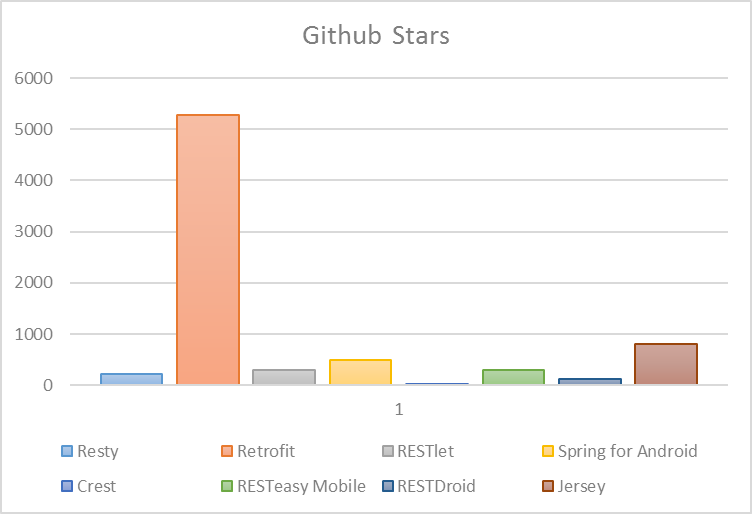
\includegraphics[width=0.8\textwidth]{imgs/github_stars.png}}
	\subfigure[Diagramm: Github Commits]{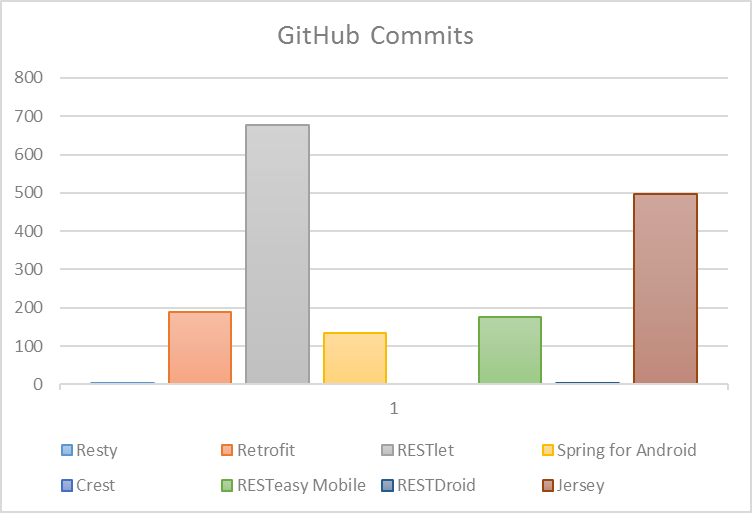
\includegraphics[width=0.8\textwidth]{imgs/github_commits.png}}
	\caption{Github Statistiken}	
	\label{figure:github}
\end{figure}

Es würde den Rahmen der Bachelorarbeit sprengen alle REST Frameworks zu evaluieren, deswegen werden nur die populärsten drei ausgewählt. Diese wurden mithilfe von Github ermittelt, indem zu einem die Github Stars mit den Commits (seit dem 01.01.2014)  in den Repositories verglichen wurden, siehe Abbildung \ref{figure:github}. Es werden daher folgende REST-Frameworks evaluiert und miteinander verglichen:

\begin{itemize}
	\item Retrofit 
	\item Jersey
	\item Spring for Android
\end{itemize}

%=======================================================================
\section{Inhaltsverzeichnis}
%=======================================================================
Geplante Struktur der Arbeit: ca. 40 Seiten	
\begin{samepage}
  \begin{contentstructure}
    \item Einleitung	\estimatedpages{3 Seiten}
    \item State of the Art \estimatedpages{8 Seiten}
    \begin{contentstructure}
      \item Auswahl der Frameworks \estimatedpages{3 Seiten}
      \item Beschreibung der Frameworks \estimatedpages{5 Seiten}
    \end{contentstructure}
    \item Android \estimatedpages{7 Seiten}
    \begin{contentstructure}
      \item Aufbau \estimatedpages{2 Seiten}
      \item Prozess der App Implementierung \estimatedpages{5 Seiten}
    \end{contentstructure}
    \item Evaluierung der Frameworks \estimatedpages{9 Seiten}
    \begin{contentstructure}
      \item Framework 1	\estimatedpages{3 Seiten}
      \item Framework 2 \estimatedpages{3 Seiten}
      \item Framework 3 \estimatedpages{3 Seiten}
    \end{contentstructure}
    \item Ergebnis \estimatedpages{3 Seiten}
    \item Zusammenfassung \estimatedpages{2 Seiten}
  \end{contentstructure}
\end{samepage}

%=======================================================================
\section{Zeitplan}
%=======================================================================
Zeitplanung der geplanten Arbeit mit wichtigen Meilensteine.

\begin{spacing}{1.4}
\begin{longtable}{|p{.2 \linewidth}|p{.5 \linewidth}|}
	\hline
	\multicolumn{1}{|c|}{\textbf{Zeitraum}} & \textbf{Phase} \\ 
	\hline 
	Mitte Mai & Schreiben des Exposé \\ 
	\hline 
	Mitte Mai & Auswahl der Frameworks \\
	\hline 
	ab Mitte Mai & Erstellung der App mit ersten Framework \\
	\hline 
	Juni & Evaluierung der restlichen Frameworks \\
	\hline 
	Juni- Ende Juli & Schreiben des theoretischen Teils \\
	\hline
	\caption{Zeitplan}
	\label{tab:tabZeitplan}
\end{longtable}
\end{spacing}

\newpage
\nocite{dobjanschi:developing-android}
\nocite{tilko:rest}
\nocite{louis:android}
\nocite{stackOverflow:rest-client}
\nocite{burd:android}
% Bibliographie
\printbibliography

\end{document}
